\section{Reference}
\label{sec:reference}

\subsection{Common Syntax}
\label{sec:common-syntax}
\begin{center}
  \begin{Bcode}
ML_COMMENT ::= /* STRING */\\
SL_COMMENT ::= // SL_STRING \\
ID ::= [^] (LETTER | \_) \{LETTER | DIGIT | \_ \}\\
XLABEL ::= @STRING:\\
  \end{Bcode}
\end{center}


\subsection{XContext Syntax}
\label{sec:xcontext-syntax}

\begin{center}
  \begin{Bcode}
    XCONTEXT ::= \\
    \Btab \Btab [ ML_COMMENT | SL_COMMENT ]\\
    \Btab \Btab \Bcontext{} ID \\
    \Btab \Btab [\Bextends{} ID \{ ID \}]\\
    \Btab \Btab [\Bsets{} XSET \{XSET\}]\\
    \Btab \Btab [\Bconstants{} XCONSTANT \{ XCONSTANT \}]\\
    \Btab \Btab [\Baxioms{} XAXIOM \{XAXIOM\}]\\[2ex]
    \Btab \Btab \Bend\\
    XSET ::= \\
    \Btab \Btab XSET\_NO\_COMMENT | \\
    \Btab \Btab XSET\_ML\_COMMENT | \\
    \Btab \Btab XSET\_SL\_COMMENT \\
    XSET\_NO\_COMMENT ::= ID \\
    XSET\_ML\_COMMENT ::= ML\_COMMENT ID\\
    XSET\_SL\_COMMENT ::= ID ML\_COMMENT\\
    XCONSTANT ::= \\
    \Btab \Btab XCONSTANT\_NO\_COMMENT | \\
    \Btab \Btab XCONSANT\_ML\_COMMENT | \\
    \Btab \Btab XCONSTANT\_SL\_COMMENT \\
    XCONSTANT\_NO\_COMMENT ::= ID \\
    XCONSTANT\_ML\_COMMENT ::= ML\_COMMENT ID\\
    XCONSTANT\_SL\_COMMENT ::= ID ML\_COMMENT\\
    XAXIOM ::= \\
    \Btab \Btab XAXIOM\_NO\_COMMENT | \\
    \Btab \Btab XAXIOM\_ML\_COMMENT | \\
    \Btab \Btab XAXIOM\_SL\_COMMENT \\
    XAXIOM\_NO\_COMMENT ::= XLABEL "XPREDICATE" [\Btheorem]\\
    XAXIOM\_ML\_COMMENT ::= ML\_COMMENT XLABEL "XPREDICATE" [\Btheorem]\\
    XAXIOM\_SL\_COMMENT ::= XLABEL "XPREDICATE" [\Btheorem] SL\_COMMENT\\
  \end{Bcode}
\end{center}

\subsection{XMachine syntax}
\label{sec:xmachine-syntax}
\begin{center}
  \begin{Bcode}
    XMACHINE ::= [ ML_COMMENT | SL_COMMENT ]\\
    \Btab \Btab \Bmachine{} ID \\
    \Btab \Btab [\Brefines{} ID\\
    \Btab \Btab [\Bsees{} ID \{ ID \}\\
    \Btab \Btab [\Bvariables{} XVARIABLE \{XVARIABLE\}]\\
    \Btab \Btab [\Binvariants{} XINVARIANT \{ XINVARIANT \}]\\
    \Btab \Btab [\Bvariant{} XVARIANT]\\
    \Btab \Btab [\Bevents{} XEVENT \{ XEVENT \}] \\
    \Btab \Btab \Bend \\
    XVARIABLE ::= \\
    \Btab \Btab XVARIABLE\_NO\_COMMENT | \\
    \Btab \Btab XVARIABLE\_ML\_COMMENT | \\
    \Btab \Btab XVARIABLE\_SL\_COMMENT \\
    XVARIABLE\_NO\_COMMENT ::= ID \\
    XVARIABLE\_ML\_COMMENT ::= ML\_COMMENT ID \\
    XVARIABLE\_SL\_COMMENT ::= ID SL\_COMMENT \\
    XINVARIANT ::=\\
    \Btab \Btab XINVARIANT\_NO\_COMMENT\\
    \Btab \Btab XINVARIANT\_ML\_COMMENT\\
    \Btab \Btab XINVARIANT\_SL\_COMMENT\\
    XINVARIANT\_NO\_COMMENT ::= \\
    \Btab \Btab XLABEL "XPREDICATE" [\Btheorem] \\
    XINVARIANT\_ML\_COMMENT ::= \\
    \Btab \Btab ML\_COMMENT XLABEL "XPREDICATE" [\Btheorem]\\
    XINVARIANT\_SL\_COMMENT ::= \\
    \Btab \Btab XLABEL "XPREDICATE" [\Btheorem] SL\_COMMENT\\
    XEVENT ::= \\
    \Btab \Btab XEVENT\_NO\_COMMENT\\
    \Btab \Btab XEVENT\_ML\_COMMENT\\
    \Btab \Btab XEVENT\_SL\_COMMENT\\
    XEVENT\_NO\_COMMENT ::=\\
    \Btab \Btab ID \\
    \Btab \Btab ([\Bextended] \& [\Bordinary | \Bconvergent | \Banticipated])\\
    \Btab \Btab [\Brefines{} ID \{ ID \}]\\
    \Btab \Btab [\\
    \Btab \Btab \Btab [\Bwith{} XWITNESS \{ XWITNESS \}] \\
    \Btab \Btab \Btab \Bbegin{} XACTION \{ XACTION \} \\
    \Btab \Btab \Btab | \\
    \Btab \Btab \Btab \Bwhen{} XGUARD \{ XGUARD \}\\
    \Btab \Btab \Btab [\Bwith{} XWITNESS \{ XWITNESS \}] \\
    \Btab \Btab \Btab [\Bthen{} XACTION \{ XACTION \}] \\
    \Btab \Btab \Btab | \\
    \Btab \Btab \Btab \Bany{} XPARAMETER \{ XPARAMETER \}\\
    \Btab \Btab \Btab \Bwhere{} XGUARD \{ XGUARD \}\\
    \Btab \Btab \Btab [\Bwith{} XWITNESS \{ XWITNESS \}] \\
    \Btab \Btab \Btab [\Bthen{} XACTION \{ XACTION \}] \\
    \Btab \Btab ]\\
    \Btab \Btab \Bend\\
    XEVENT\_ML\_COMMENT ::=\\
    \Btab \Btab ML\_COMMENT\\
    \Btab \Btab ID \\
    \Btab \Btab ([\Bextended] \& [\Bordinary | \Bconvergent | \Banticipated])\\
    \Btab \Btab [\Brefines{} ID \{ ID \}]\\
    \Btab \Btab [\\
    \Btab \Btab \Btab [\Bwith{} XWITNESS \{ XWITNESS \}] \\
    \Btab \Btab \Btab \Bbegin{} XACTION \{ XACTION \} \\
    \Btab \Btab \Btab | \\
    \Btab \Btab \Btab \Bwhen{} XGUARD \{ XGUARD \}\\
    \Btab \Btab \Btab [\Bwith{} XWITNESS \{ XWITNESS \}] \\
    \Btab \Btab \Btab [\Bthen{} XACTION \{ XACTION \}] \\
    \Btab \Btab \Btab | \\
    \Btab \Btab \Btab \Bany{} XPARAMETER \{ XPARAMETER \}\\
    \Btab \Btab \Btab \Bwhere{} XGUARD \{ XGUARD \}\\
    \Btab \Btab \Btab [\Bwith{} XWITNESS \{ XWITNESS \}] \\
    \Btab \Btab \Btab [\Bthen{} XACTION \{ XACTION \}] \\
    \Btab \Btab ]\\
    \Btab \Btab \Bend\\
    XEVENT\_SL\_COMMENT ::=\\
    \Btab \Btab ID \\
    \Btab \Btab ([\Bextended] \& [\Bordinary | \Bconvergent | \Banticipated])\\
    \Btab \Btab [\Brefines{} ID \{ ID \}]\\
    \Btab \Btab SL\_COMMENT\\
    \Btab \Btab [\\
    \Btab \Btab \Btab [\Bwith{} XWITNESS \{ XWITNESS \}] \\
    \Btab \Btab \Btab \Bbegin{} XACTION \{ XACTION \} \\
    \Btab \Btab \Btab | \\
    \Btab \Btab \Btab \Bwhen{} XGUARD \{ XGUARD \}\\
    \Btab \Btab \Btab [\Bwith{} XWITNESS \{ XWITNESS \}] \\
    \Btab \Btab \Btab [\Bthen{} XACTION \{ XACTION \}] \\
    \Btab \Btab \Btab | \\
    \Btab \Btab \Btab \Bany{} XPARAMETER \{ XPARAMETER \}\\
    \Btab \Btab \Btab \Bwhere{} XGUARD \{ XGUARD \}\\
    \Btab \Btab \Btab [\Bwith{} XWITNESS \{ XWITNESS \}] \\
    \Btab \Btab \Btab [\Bthen{} XACTION \{ XACTION \}] \\
    \Btab \Btab ]\\
    \Btab \Btab \Bend\\
    XWITNESS ::= \\
    \Btab \Btab XWITNESS\_NO\_COMMENT | \\
    \Btab \Btab XWITNESS\_ML\_COMMENT | \\
    \Btab \Btab XWITNESS\_SL\_COMMENT | \\
    XWITNESS\_NO\_COMMENT ::= XLABEL "XPREDICATE" \\
    XWITNESS\_ML\_COMMENT ::= ML\_COMMENT XLABEL "XPREDICATE" \\
    XWITNESS\_SL\_COMMENT ::= XLABEL "XPREDICATE" SL\_COMMENT \\
    XPARAMETER ::= \\
    \Btab \Btab XPARAMETER\_NO\_COMMENT | \\
    \Btab \Btab XPARAMETER\_ML\_COMMENT | \\
    \Btab \Btab XPARAMETER\_SL\_COMMENT \\
    XPARAMETER\_NO\_COMMENT ::= ID \\
    XPARAMETER\_ML\_COMMENT ::= ML\_COMMENT ID \\
    XPARAMETER\_SL\_COMMENT ::= ID SL\_COMMENT \\
    XGUARD ::=\\
    \Btab \Btab XGUARD\_NO\_COMMENT |\\
    \Btab \Btab XGUARD\_ML\_COMMENT |\\
    \Btab \Btab XGUARD\_SL\_COMMENT\\
    XGUARD\_NO\_COMMENT ::= \\
    \Btab \Btab XLABEL "XPREDICATE" [\Btheorem]\\
    XGUARD\_ML\_COMMENT ::= \\
    \Btab \Btab ML\_COMMENT XLABEL "XPREDICATE" [\Btheorem]\\
    XGUARD\_SL\_COMMENT ::= \\
    \Btab \Btab XLABEL "XPREDICATE" [\Btheorem] SL\_COMMENT\\
    XACTION ::=\\
    \Btab \Btab XACTION\_NO\_COMMENT |\\
    \Btab \Btab XACTION\_ML\_COMMENT |\\
    \Btab \Btab XACTION\_SL\_COMMENT\\
    XACTION\_NO\_COMMENT ::= XLABEL "XASSIGNMENT" [\Btheorem]\\
    XACTION\_ML\_COMMENT ::= ML\_COMMENT XLABEL "XASSIGNMENT"\\
    XACTION\_SL\_COMMENT ::= XLABEL "XASSIGNMENT" SL\_COMMENT
  \end{Bcode}
\end{center}

\subsection{Preferences}
\label{sec:preferences}

\subsubsection{XContext Preferences}
\label{sec:xcontext-preferences}
The following XContext preferences can be set on the  the XContext preference page and its sub-pages.

\paragraph{Compiler}
\begin{table}[!htbp]
  \centering
  \begin{tabular}{|p{0.2\textwidth}|p{0.5\textwidth}|p{0.3\textwidth}|}
    \hline
    \multicolumn{1}{|c}{\textbf{Option}} & \multicolumn{1}{|c}{\textbf{Description}} &%
                                                                                       \multicolumn{1}{|c|}{\textbf{Default}} \\
    \hline
    Compiler is activated & \textbf{Compiler is activated} or \textbf{deactivated} & Activated \\
    \hline
  \end{tabular}
  \caption{XContext Compiler Preferences}
  \label{tab:xcontext-compiler-preference}
\end{table}

\paragraph{Syntax Coloring}
\begin{table}[!htbp]
  \centering
  \begin{tabular}{|p{0.2\textwidth}|p{0.5\textwidth}|p{0.3\textwidth}|}
    \hline
    \multicolumn{1}{|c}{\textbf{Option}} & \multicolumn{1}{|c}{\textbf{Description}} &%
                                                                                       \multicolumn{1}{|c|}{\textbf{Default}} \\
    \hline
    Comment & \textbf{Color} & Dark Green \\
                                         & \textbf{Background} & White \\
                                         & \textbf{Style} (Italic, Bold, Underline, Strike through) & None \\
                                         & \textbf{Font} & Platform dependent \\
    \hline
    Default & \textbf{Color} & Black \\
                                         & \textbf{Background} & White \\
                                         & \textbf{Style} (Italic, Bold, Underline, Strike through) & None \\
                                         & \textbf{Font} & Platform dependent \\
    \hline
    Invalid Symbol & \textbf{Color} & Black \\
                                         & \textbf{Background} & White \\
                                         & \textbf{Style} (Italic, Bold, Underline, Strike through) & None \\
                                         & \textbf{Font} & Platform dependent \\
    \hline
    Keyword & \textbf{Color} & Dark Purple \\
                                         & \textbf{Background} & White \\
                                         & \textbf{Style} (Italic, Bold, Underline, Strike through) & Bold \\
                                         & \textbf{Font} & Platform dependent \\
    \hline
    Number & \textbf{Color} & Dark Gray \\
                                         & \textbf{Background} & White \\
                                         & \textbf{Style} (Italic, Bold, Underline, Strike through) & None \\
                                         & \textbf{Font} & Platform dependent \\
    \hline
    Punctuation character & \textbf{Color} & Black \\
                                         & \textbf{Background} & White \\
                                         & \textbf{Style} (Italic, Bold, Underline, Strike through) & None \\
                                         & \textbf{Font} & Platform dependent \\
    \hline
    String & \textbf{Color} & Blue \\
                                         & \textbf{Background} & White \\
                                         & \textbf{Style} (Italic, Bold, Underline, Strike through) & None \\
                                         & \textbf{Font} & Platform dependent \\
    \hline
    Task Tag & \textbf{Color} & Light Blue \\
                                         & \textbf{Background} & White \\
                                         & \textbf{Style} (Italic, Bold, Underline, Strike through) & Bold \\
                                         & \textbf{Font} & Platform dependent \\
    \hline
  \end{tabular}
  \caption{XContext Syntax Coloring Preferences}
  \label{tab:xcontext-syntax-coloring-preference}
\end{table}


\subsubsection{XMachine Preferences}
\label{sec:xmachine-preferences}
The following XMachine preferences can be set on the  XMachine preference page and its sub-pages.

\paragraph{Compiler}
\begin{table}[!htbp]
  \centering
  \begin{tabular}{|p{0.2\textwidth}|p{0.5\textwidth}|p{0.3\textwidth}|}
    \hline
    \multicolumn{1}{|c}{\textbf{Option}} & \multicolumn{1}{|c}{\textbf{Description}} &%
                                                                                       \multicolumn{1}{|c|}{\textbf{Default}} \\
    \hline
    Compiler is activated & \textbf{Compiler is activated} or \textbf{deactivated} & Activated \\
    \hline
  \end{tabular}
  \caption{XMachine Compiler Preferences}
  \label{tab:xmachine-compiler-preference}
\end{table}

\paragraph{Syntax Coloring}
\begin{table}[!htbp]
  \centering
  \begin{tabular}{|p{0.2\textwidth}|p{0.5\textwidth}|p{0.3\textwidth}|}
    \hline
    \multicolumn{1}{|c}{\textbf{Option}} & \multicolumn{1}{|c}{\textbf{Description}} &%
                                                                                       \multicolumn{1}{|c|}{\textbf{Default}} \\
    \hline
    Comment & \textbf{Color} & Dark Green \\
                                         & \textbf{Background} & White \\
                                         & \textbf{Style} (Italic, Bold, Underline, Strike through) & None \\
                                         & \textbf{Font} & Platform dependent \\
    \hline
    Default & \textbf{Color} & Black \\
                                         & \textbf{Background} & White \\
                                         & \textbf{Style} (Italic, Bold, Underline, Strike through) & None \\
                                         & \textbf{Font} & Platform dependent \\
    \hline
    Invalid Symbol & \textbf{Color} & Black \\
                                         & \textbf{Background} & White \\
                                         & \textbf{Style} (Italic, Bold, Underline, Strike through) & None \\
                                         & \textbf{Font} & Platform dependent \\
    \hline
    Keyword & \textbf{Color} & Dark Purple \\
                                         & \textbf{Background} & White \\
                                         & \textbf{Style} (Italic, Bold, Underline, Strike through) & Bold \\
                                         & \textbf{Font} & Platform dependent \\
    \hline
    Number & \textbf{Color} & Dark Gray \\
                                         & \textbf{Background} & White \\
                                         & \textbf{Style} (Italic, Bold, Underline, Strike through) & None \\
                                         & \textbf{Font} & Platform dependent \\
    \hline
    Punctuation character & \textbf{Color} & Black \\
                                         & \textbf{Background} & White \\
                                         & \textbf{Style} (Italic, Bold, Underline, Strike through) & None \\
                                         & \textbf{Font} & Platform dependent \\
    \hline
    String & \textbf{Color} & Blue \\
                                         & \textbf{Background} & White \\
                                         & \textbf{Style} (Italic, Bold, Underline, Strike through) & None \\
                                         & \textbf{Font} & Platform dependent \\
    \hline
    Task Tag & \textbf{Color} & Light Blue \\
                                         & \textbf{Background} & White \\
                                         & \textbf{Style} (Italic, Bold, Underline, Strike through) & Bold \\
                                         & \textbf{Font} & Platform dependent \\
    \hline
  \end{tabular}
  \caption{XMachine Syntax Coloring Preferences}
  \label{tab:xmachine-syntax-coloring-preference}
\end{table}

\subsection{XEvent-B Editors}
\label{sec:xevent-b-editors}


\subsubsection{XEvent-B Content Assist}
\label{sec:xevent-b-content}
In the XContext and XMachine editors press \texttt{Ctrl+Space} on code to complete. This opens a list of available code completions. Some tips for using code assist are listed in the following paragraph:
\begin{itemize}
\item You can use the mouse or the keyboard (Up Arrow, Down Arrow, Page Up, Page Down, Home, End, Enter) to navigate and select lines in the list.

\item Clicking or pressing Enter on a selected line in the list inserts the selection into the editor.
\end{itemize}
\begin{figure}[!htbp]
  \centering
  \ifplastex
  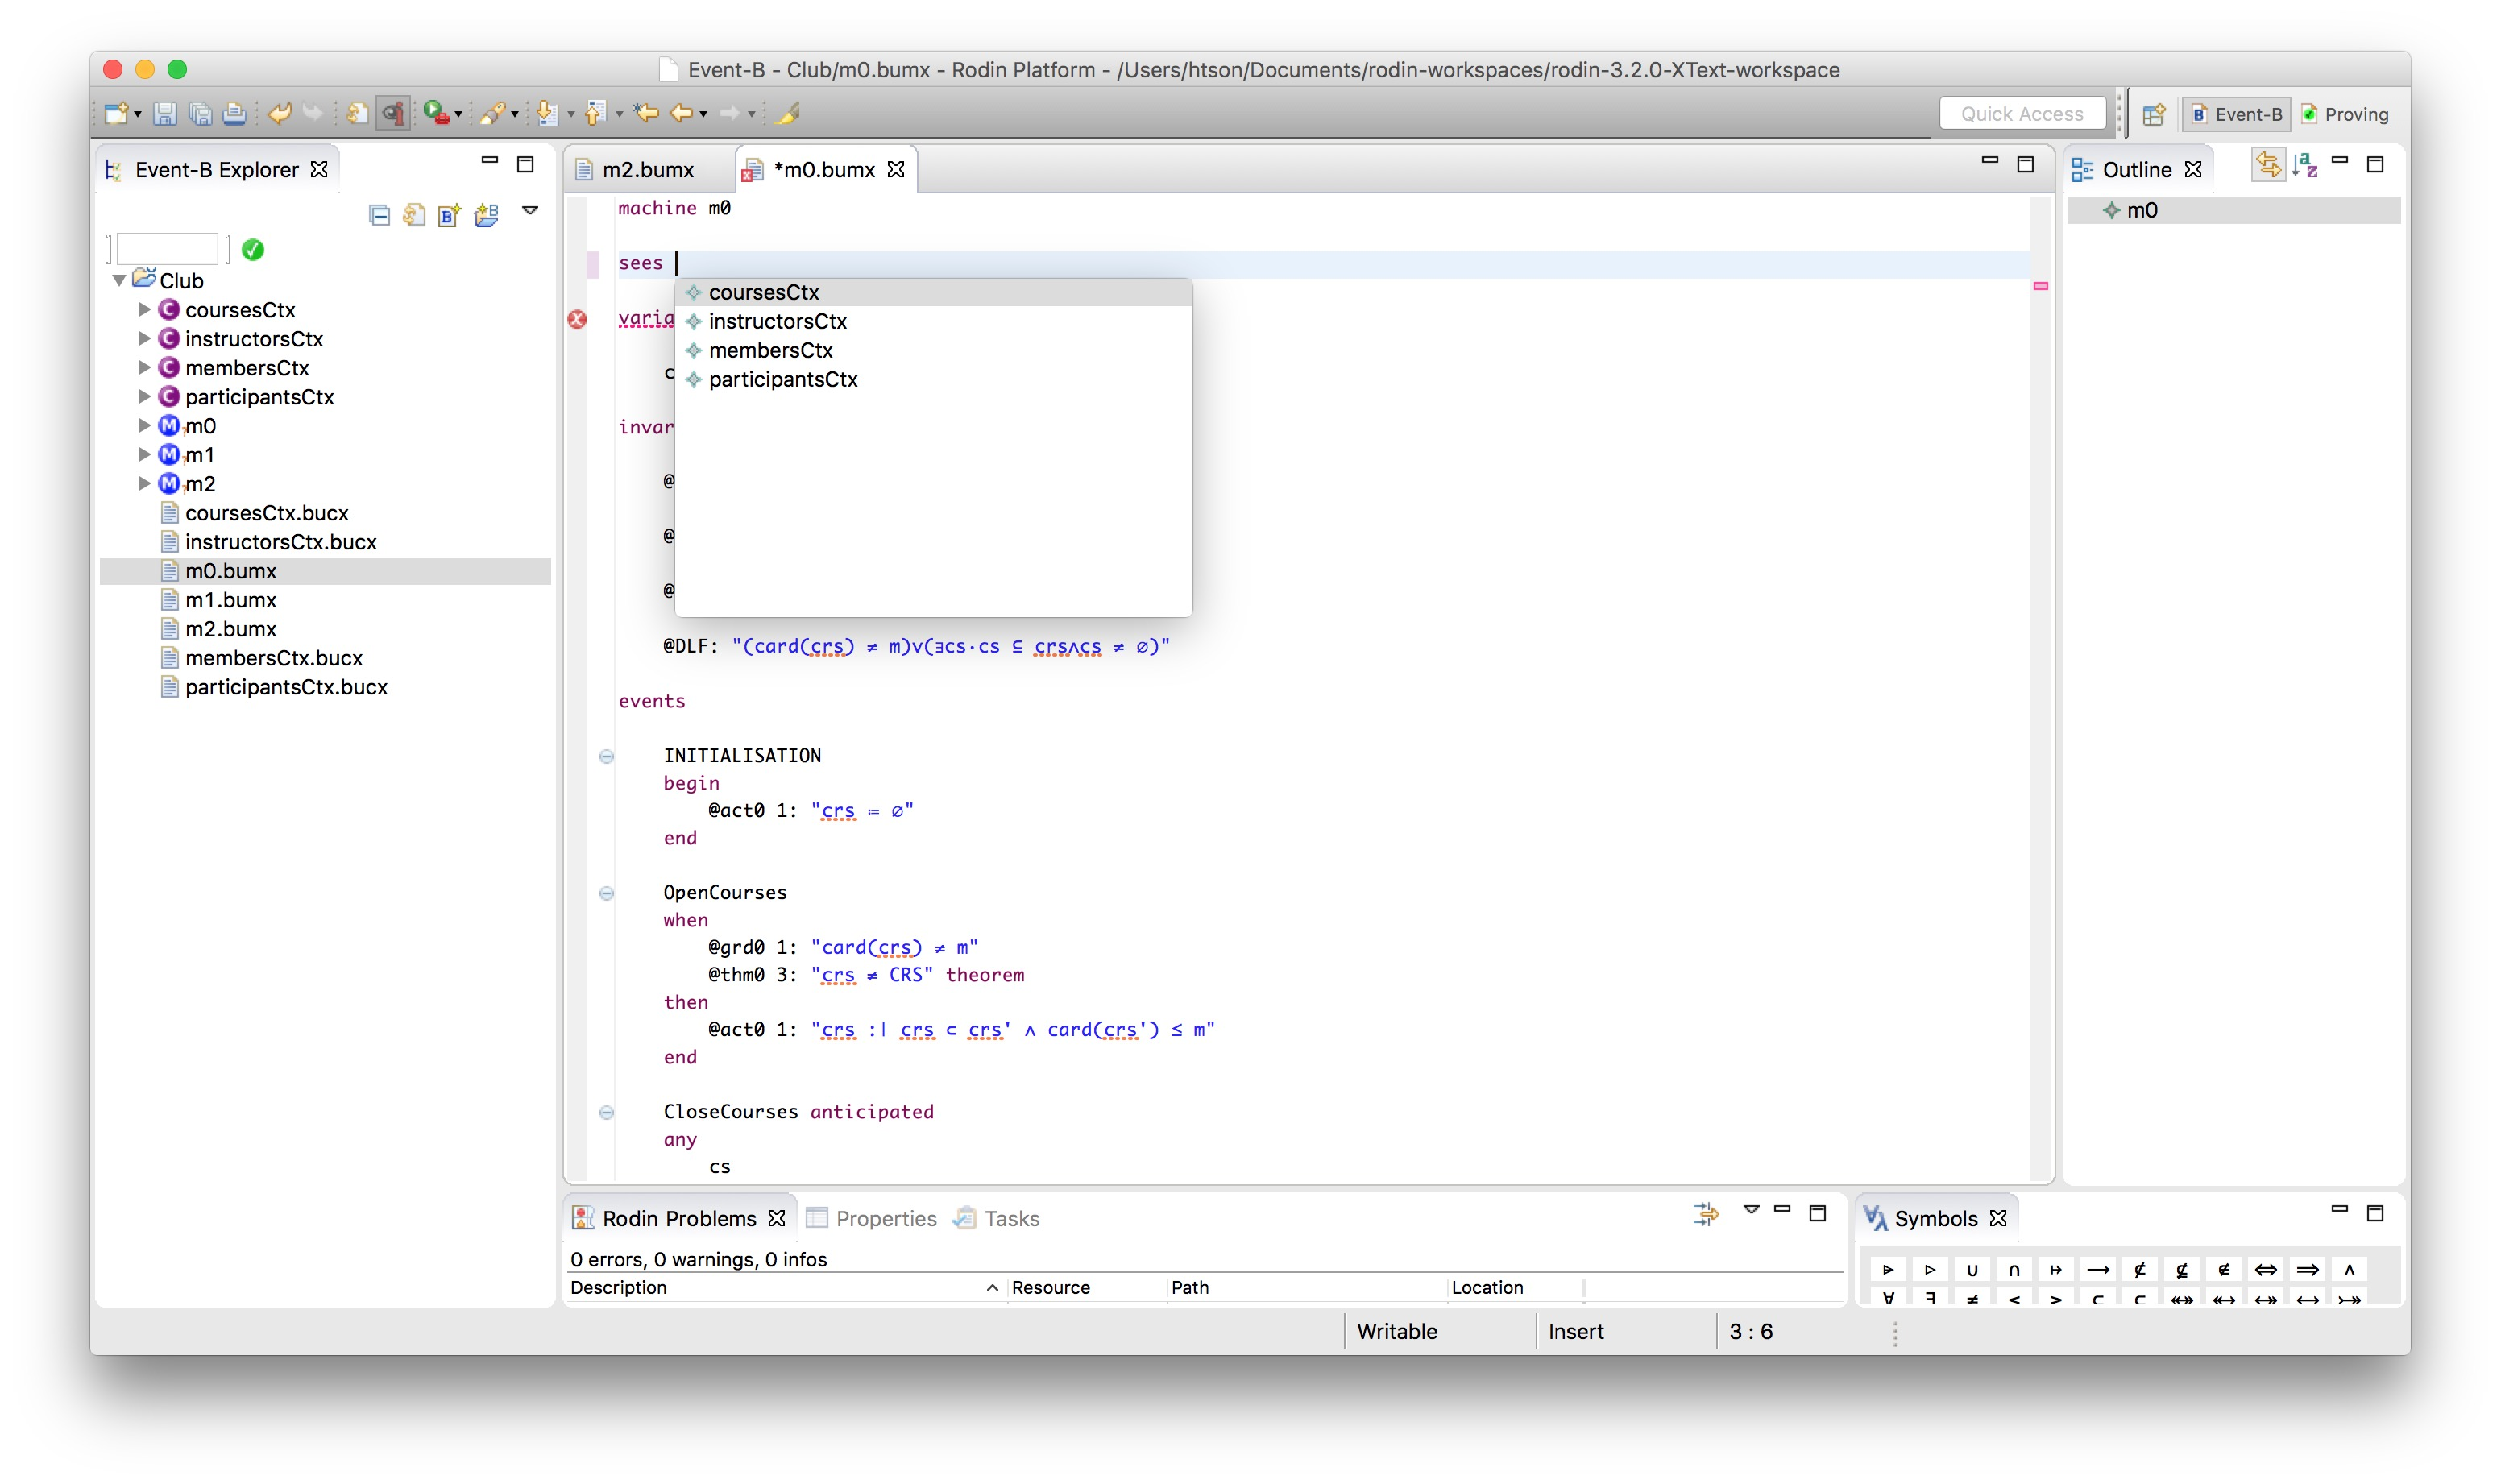
\includegraphics[width=512]{figures/SeesContentAssist}
  \else
  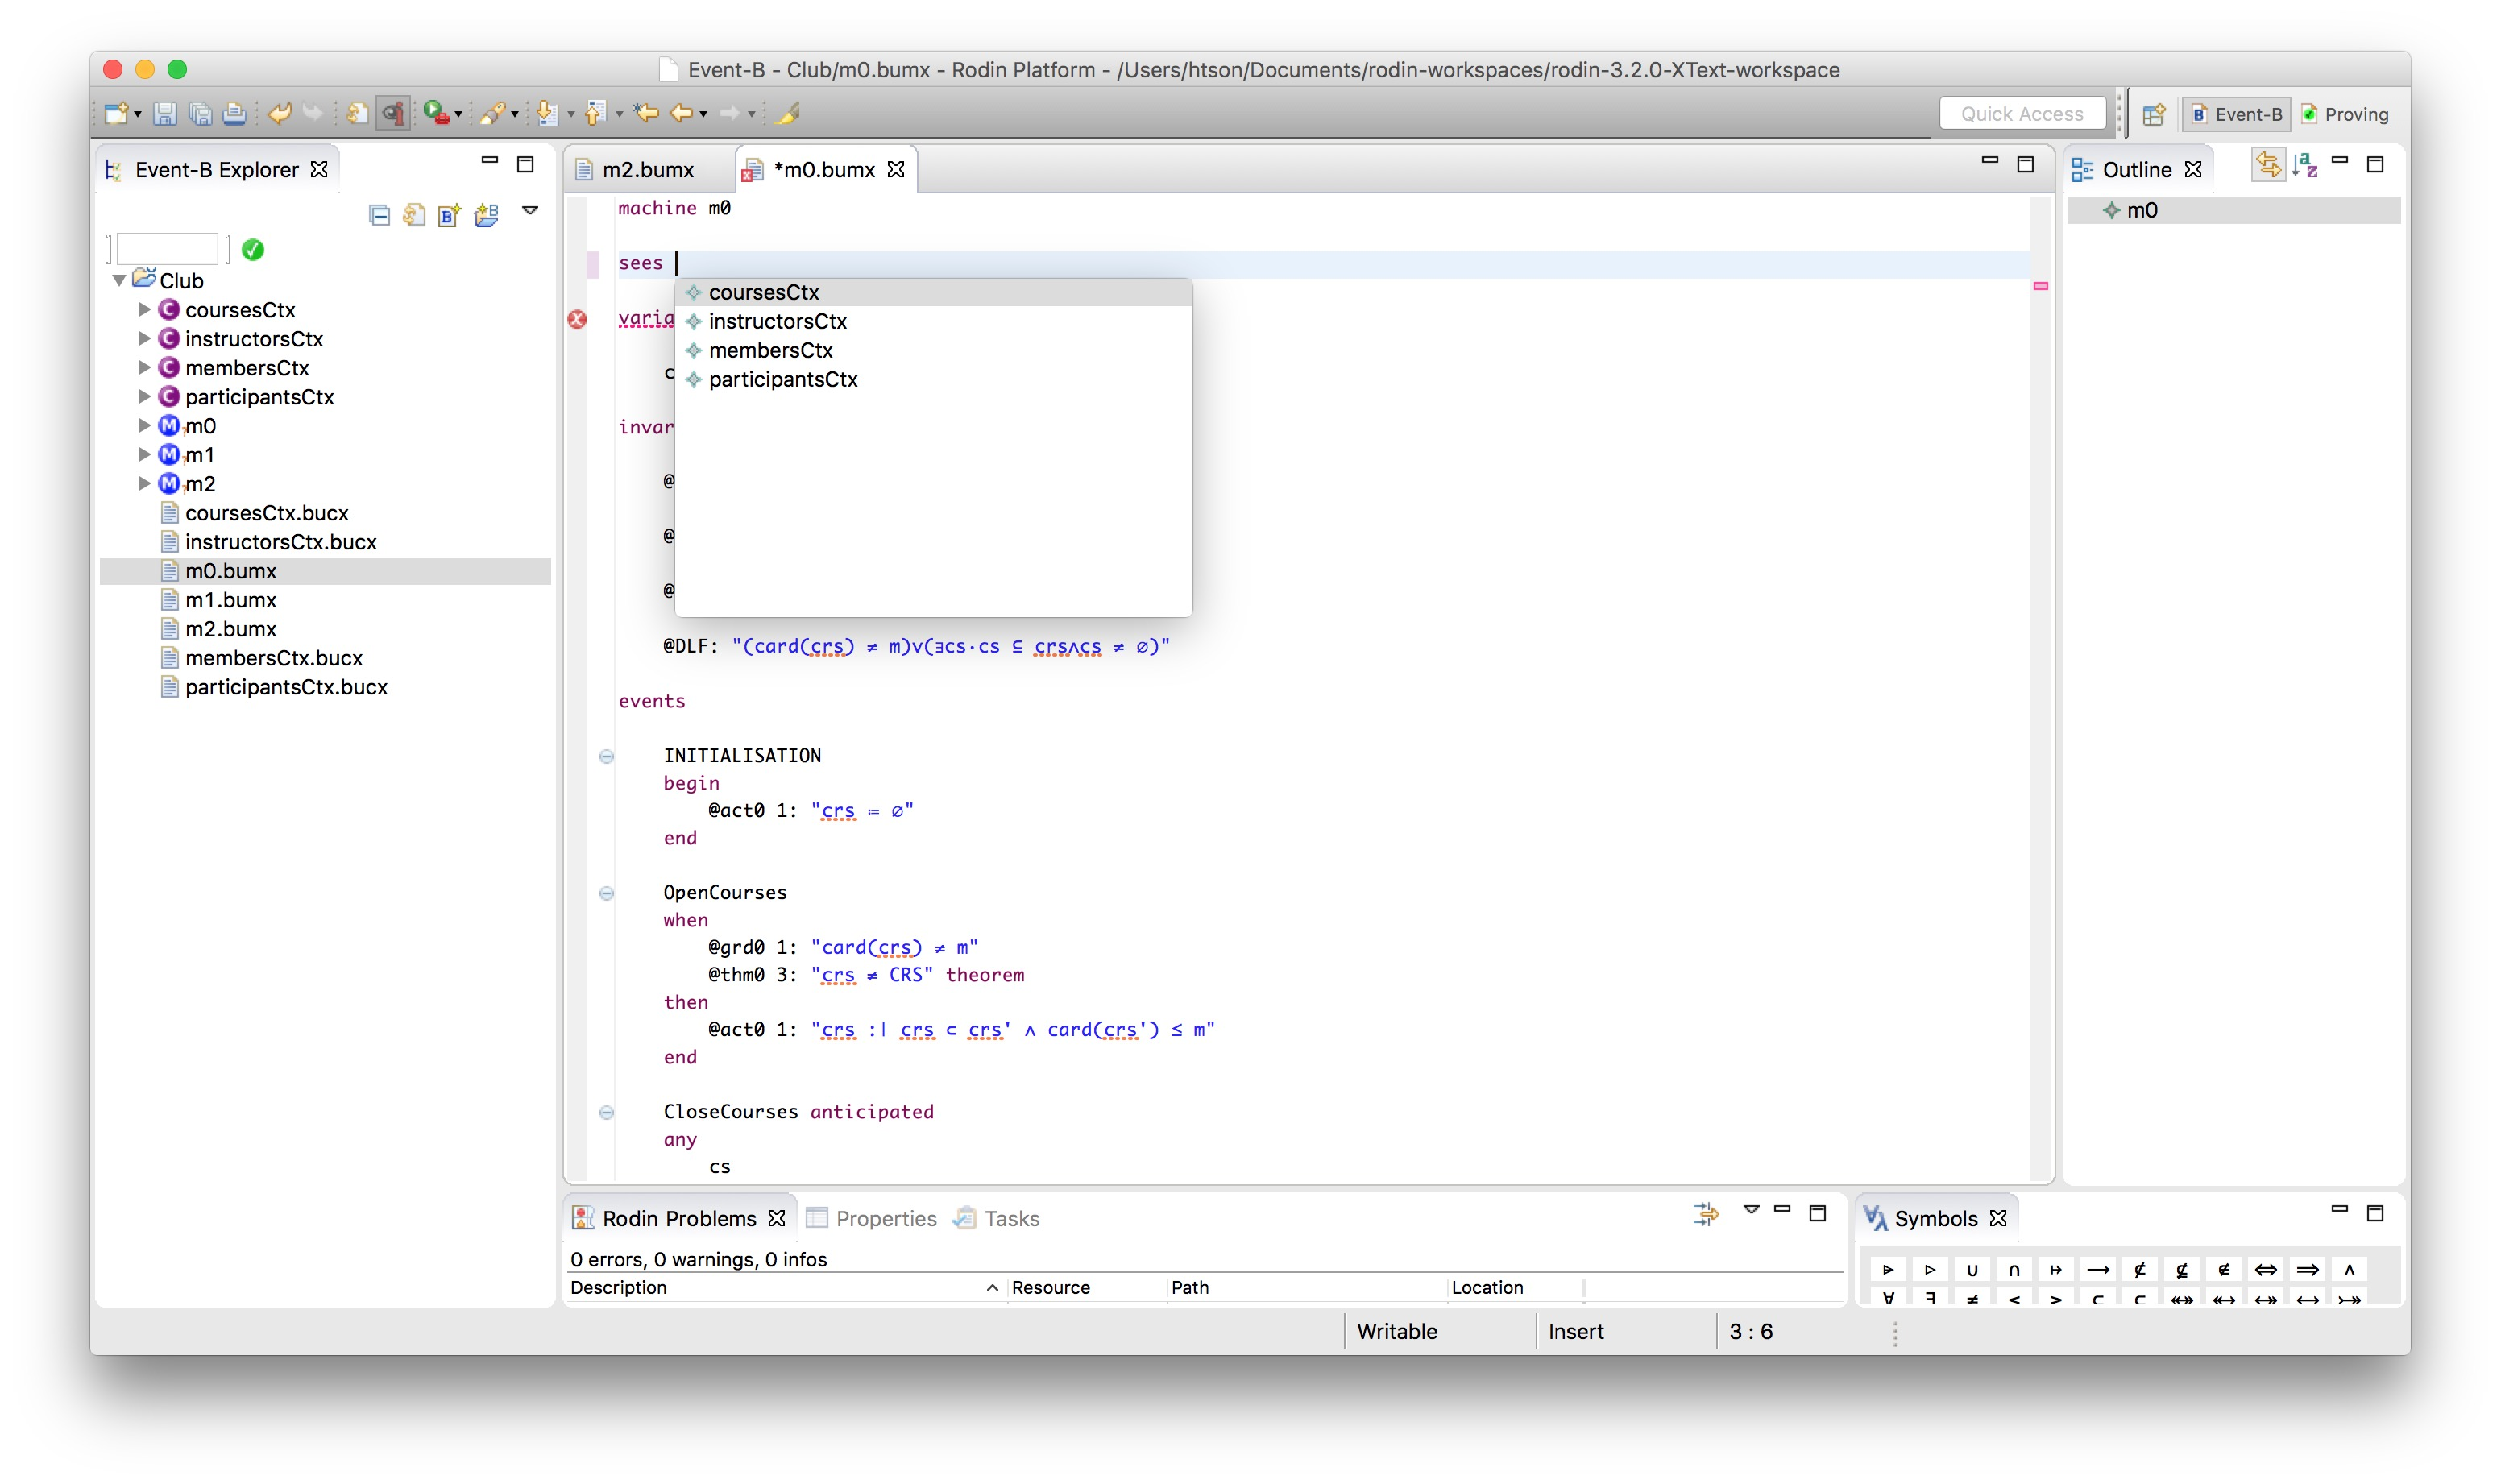
\includegraphics[width=0.9\textwidth]{figures/SeesContentAssist}
  \fi
  \caption{Content Assist for adding Sees clause}
  \label{fig:SeesContentAssist}
\end{figure}

\subsubsection{XEvent-B Formatter}
\label{sec:xevent-b-formatter}
In the XContent and XMachine editors press \texttt{Ctrl+Shift+F} on code to format it. If no selection is set then the entire source is formatted otherwise only the selection will be. 

%%% Local Variables:
%%% mode: latex
%%% TeX-master: "user_manual"
%%% End:
